\section{Date: 2026-09-14}
\noindent \textbf{Series ID: ATNHPIUS37100Q} 

\noindent This series is titled All-Transactions House Price Index for Oxnard-Thousand Oaks-Ventura, CA (MSA) and has a frequency of Quarterly. The units are Index 1995:Q1=100 and the seasonal adjustment is Not Seasonally Adjusted.The observation start date is 1976-04-01 and the observation end date is 2026-04-01.The popularity of this series is 6. \\ 

\noindent \textbf{Series ID: FBGFIEQ027S} 

\noindent This series is titled Financial business; gross fixed investment, nonresidential equipment, software, and structures, Flow (DISCONTINUED) and has a frequency of Quarterly. The units are Millions of Dollars and the seasonal adjustment is Seasonally Adjusted Annual Rate.The observation start date is 1946-10-01 and the observation end date is 2017-10-01.The popularity of this series is 1. \\ 

\subsection{Raw Regression}
\noindent Regresses the two series against each other directly. A significant result here can come just as easily from both series sharing a long-run trend as from any real relationship.

\begin{center}
\begin{tabular}{lclc}
\toprule
\textbf{Dep. Variable:}              & value\_fred\_FBGFIEQ027S & \textbf{  R-squared:         } &     0.870   \\
\textbf{Model:}                      &           OLS            & \textbf{  Adj. R-squared:    } &     0.869   \\
\textbf{Method:}                     &      Least Squares       & \textbf{  F-statistic:       } &     1103.   \\
\textbf{Date:}                       &     Mon, 14 Sep 2026     & \textbf{  Prob (F-statistic):} &  5.84e-75   \\
\textbf{Time:}                       &         17:07:08         & \textbf{  Log-Likelihood:    } &   -1926.0   \\
\textbf{No. Observations:}           &             167          & \textbf{  AIC:               } &     3856.   \\
\textbf{Df Residuals:}               &             165          & \textbf{  BIC:               } &     3862.   \\
\textbf{Df Model:}                   &               1          & \textbf{                     } &             \\
\textbf{Covariance Type:}            &        nonrobust         & \textbf{                     } &             \\
\bottomrule
\end{tabular}
\begin{tabular}{lcccccc}
                                     & \textbf{coef} & \textbf{std err} & \textbf{t} & \textbf{P$> |$t$|$} & \textbf{[0.025} & \textbf{0.975]}  \\
\midrule
\textbf{const}                       &    1.341e+04  &     3837.676     &     3.493  &         0.001        &     5829.236    &      2.1e+04     \\
\textbf{value\_fred\_ATNHPIUS37100Q} &     745.7296  &       22.457     &    33.207  &         0.000        &      701.389    &      790.070     \\
\bottomrule
\end{tabular}
\begin{tabular}{lclc}
\textbf{Omnibus:}       &  1.131 & \textbf{  Durbin-Watson:     } &    0.039  \\
\textbf{Prob(Omnibus):} &  0.568 & \textbf{  Jarque-Bera (JB):  } &    0.803  \\
\textbf{Skew:}          & -0.148 & \textbf{  Prob(JB):          } &    0.669  \\
\textbf{Kurtosis:}      &  3.165 & \textbf{  Cond. No.          } &     341.  \\
\bottomrule
\end{tabular}
%\caption{OLS Regression Results}
\end{center}

Notes: \newline
 [1] Standard Errors assume that the covariance matrix of the errors is correctly specified.

\begin{figure}
\centering
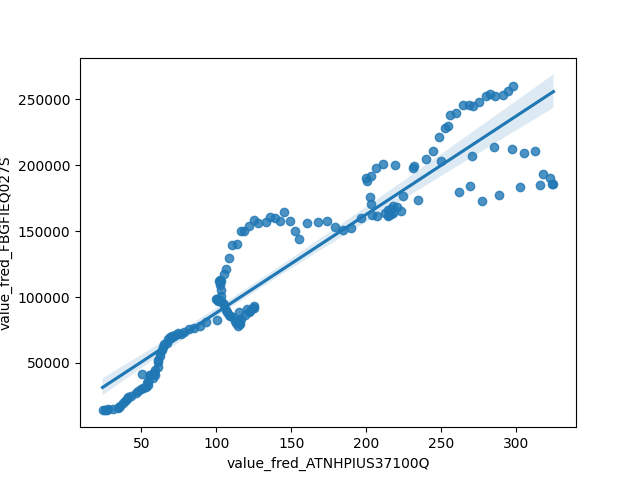
\includegraphics[scale = 0.9]{plots/plot_2026-09-14.png}
\caption{Raw Regression Plot for 2026-09-14}
\end{figure}
\newpage
\subsection{Detrended Regression}
\noindent Regresses the residuals of each series after removing its own linear time trend, so a shared trend can no longer drive the result on its own. A relationship that stays significant here is better evidence of a genuine link between the two series.

\begin{center}
\begin{tabular}{lclc}
\toprule
\textbf{Dep. Variable:}                         & value\_fred\_FBGFIEQ027S\_detrended & \textbf{  R-squared:         } &     0.233   \\
\textbf{Model:}                                 &                 OLS                 & \textbf{  Adj. R-squared:    } &     0.228   \\
\textbf{Method:}                                &            Least Squares            & \textbf{  F-statistic:       } &     50.05   \\
\textbf{Date:}                                  &           Mon, 14 Sep 2026          & \textbf{  Prob (F-statistic):} &  4.06e-11   \\
\textbf{Time:}                                  &               17:07:08              & \textbf{  Log-Likelihood:    } &   -1814.4   \\
\textbf{No. Observations:}                      &                   167               & \textbf{  AIC:               } &     3633.   \\
\textbf{Df Residuals:}                          &                   165               & \textbf{  BIC:               } &     3639.   \\
\textbf{Df Model:}                              &                     1               & \textbf{                     } &             \\
\textbf{Covariance Type:}                       &              nonrobust              & \textbf{                     } &             \\
\bottomrule
\end{tabular}
\begin{tabular}{lcccccc}
                                                & \textbf{coef} & \textbf{std err} & \textbf{t} & \textbf{P$> |$t$|$} & \textbf{[0.025} & \textbf{0.975]}  \\
\midrule
\textbf{const}                                  &   -1.573e-09  &      985.135     &  -1.6e-12  &         1.000        &    -1945.095    &     1945.095     \\
\textbf{value\_fred\_ATNHPIUS37100Q\_detrended} &     197.7479  &       27.952     &     7.075  &         0.000        &      142.559    &      252.937     \\
\bottomrule
\end{tabular}
\begin{tabular}{lclc}
\textbf{Omnibus:}       &  3.074 & \textbf{  Durbin-Watson:     } &    0.100  \\
\textbf{Prob(Omnibus):} &  0.215 & \textbf{  Jarque-Bera (JB):  } &    2.616  \\
\textbf{Skew:}          & -0.248 & \textbf{  Prob(JB):          } &    0.270  \\
\textbf{Kurtosis:}      &  3.361 & \textbf{  Cond. No.          } &     35.2  \\
\bottomrule
\end{tabular}
%\caption{OLS Regression Results}
\end{center}

Notes: \newline
 [1] Standard Errors assume that the covariance matrix of the errors is correctly specified.

\begin{figure}
\centering
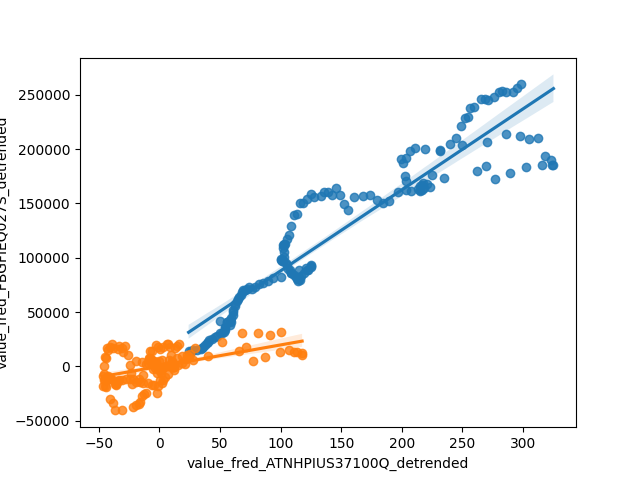
\includegraphics[scale = 0.9]{plots/plot_2026-09-14_detrended.png}
\caption{Detrended Regression Plot for 2026-09-14}
\end{figure}
\newpage
